%!TEX root = ../template.tex

\section{Introduction}
%
The understanding of the human dynamics and the way in which its contribute
 can be applied to enhance a physical
 human-robot interaction (pHRI) are two of the most promising challenges for the scientific
  community due mainly to their enormous and to-be-developed potential in industrial scenarios,
   ergonomics context, as well as in assistive and rehabilitation fields. 
Classical robots are built to act \emph{for} humans, but in order to adapt their functionality
 to the current technological progress, the new generation of robots will have to collaborate
  \emph{with} humans.  This implies that the robots will be endowed with the capability to
   control physical collaboration through intentional interaction with humans.
To achieve this condition, robots have to know mandatorily the dynamics (contact forces, internal forces,
  joint torques) of
  the human agent who they are interacting with.  However the current state of the robot 
  knowledge in
   observing human whole-body dynamics  yields to non-proficient and unadaptive interactions.
   		\\	   	   
   \indent
  To overcome this drawback, it is fundamental to understand what
   the response of the human body is while a physical interaction is
    occurring.  The importance in retrieving this information is exemplified in Fig.
	 \ref{fig:figs_schemeFrameworkLoop}: once the dynamic variables are computed by 
	 exploiting a dynamics estimation algorithm, the human dynamics feedback 
	 may be provided to the robot
	   controllers. As a consequence, the robot may adjust the strategy of interaction accordingly.
		\\	   	   
\indent
This work is the first attempt to go in this direction since a first pHRI task was
 inserted with respect to our previous work \cite{LatellaSensors2016} where only an
  investigation on the human inverse dynamics was carried out. The paper is built on the
   theoretical framework described in \cite{LatellaSensors2016} from which it inherits 
   both the notation and formulation.
   \\  
   \indent
The paper is structured as follows.  Section $2$ introduces the state-of-the-art background 
which the paper is based on.  Section $3$ presents the modelling of the human
body as an articulated multi-body system. In Section $4$ the adopted
Gaussian probabilistic domain for the sensor fusion methodology is briefly recalled.  Section $5$ outlines the 
experimental set-up followed by a description of the results in Section $6$.  
Conclusions and several considerations on the pivotal role of further control and 
estimation developments are depicted in Section $7$.
%	
\begin{figure}[ht]
  \centering
   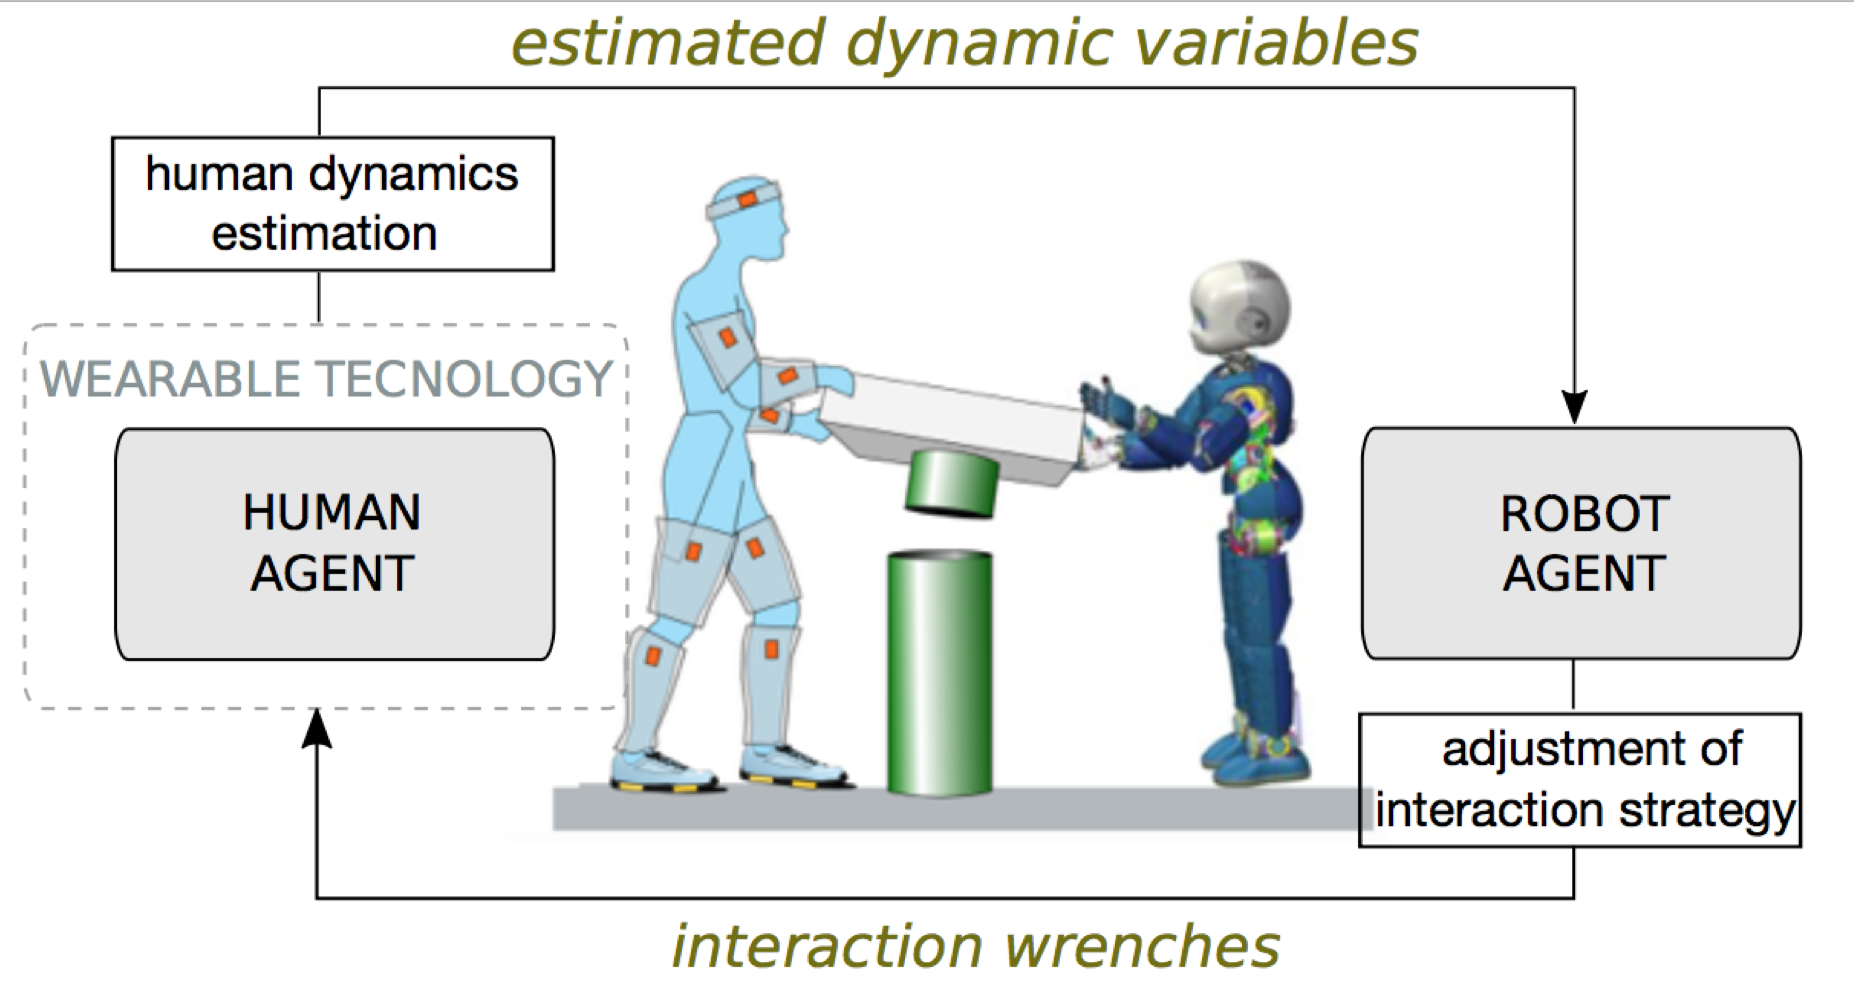
\includegraphics[width=1\columnwidth]{figs/schemeFramework}
  \caption{An example of pHRI scenario: the human agent is provided with a wearable 
  technology and an estimation algorithm allows to retrieve information about his dynamics. 
  By properly embedding estimations in the control loop of the robot, the 
  intentional collaboration may be enhanced.}
  \label{fig:figs_schemeFrameworkLoop}
\end{figure}